% 이 CVPR 템플릿 버전은 Ming-Ming Cheng에 의해 제공됩니다.
% 버그를 발견하셨다면 이슈를 남겨주세요:
% https://github.com/MCG-NKU/CVPR_Template.

%\documentclass[review]{cvpr}
\documentclass[final]{cvpr}
\usepackage{xeCJK}
\setCJKmainfont{NotoSansKR-Regular.ttf}
\setCJKsansfont{NotoSansKR-Regular.ttf}
\setCJKmonofont{NotoSansKR-Regular.ttf}
\usepackage{enumitem}
\usepackage{times}
\usepackage{epsfig}
\usepackage{graphicx}
\usepackage{amsmath}
\usepackage{amssymb}
\usepackage{makecell}
\usepackage{booktabs}
\usepackage[table,xcdraw]{xcolor}
\usepackage{multirow}
\usepackage{bbm}
\usepackage{fontspec}


% 다른 패키지를 여기에 포함시키세요, hyperref 전에.

% hyperref를 주석 처리하고 다시 주석 해제하면,
% egpaper.aux를 삭제한 후 latex를 다시 실행해야 합니다. (또는 첫 번째 latex 실행 시 'q'를 누르고,
% 완료되도록 두면 됩니다.)
\usepackage[pagebackref=true,breaklinks=true,colorlinks,bookmarks=false]{hyperref}

\def\cvprPaperID{4107} % *** 여기에 CVPR 논문 ID를 입력하세요
\def\confYear{CVPR 2021}
%\setcounter{page}{4321} % 최종 버전에서만 사용


\begin{document}

\title{철도는 기차가 아니다: 약한 지도 학습 의미론적 분할을 위한 의사-픽셀 감독으로서의 주목성}

\author{이승호\thanks{동일한 기여를 나타냅니다.}\\
연세대학교\\
{\tt\small seungholee@yonsei.ac.kr}
% 모든 저자가 동일한 기관에 있는 논문에서는,
% 다음 줄을 닫는 "}"까지 생략하세요.
% 추가 저자와 주소는 "\and"로 추가할 수 있습니다,
% 두 번째 저자와 마찬가지로.
% 공간을 절약하려면 이메일 주소나 홈페이지 중 하나만 사용하세요
\and
이민현\footnotemark[1]\\
연세대학교\\
{\tt\small lmh315@yonsei.ac.kr}
\and 
이종욱\\
성균관대학교\\
{\tt\small jongwuklee@skku.edu}
\and 
심현정\thanks{심현정은 교신 저자입니다.}\\
연세대학교\\
{\tt\small kateshim@yonsei.ac.kr}
}

\maketitle
\thispagestyle{empty}
\pagestyle{empty}

%%%%%%%%% ABSTRACT

\begin{abstract}
기존의 이미지 수준 약한 감독을 사용하는 약한 지도 학습 의미론적 분할(WSSS) 연구는 몇 가지 제한 사항이 있습니다: 희소한 객체 커버리지, 부정확한 객체 경계, 비대상 객체에서 발생하는 픽셀. 이러한 문제를 극복하기 위해, 우리는 두 가지 약한 감독을 결합하여 픽셀 수준 피드백에서 학습하는 새로운 프레임워크인 명시적 의사-픽셀 감독(EPS)을 제안합니다; 이미지 수준 레이블은 로컬라이제이션 맵을 통해 객체 정체성을 제공하고, 기성품 주목성 탐지 모델의 주목성 맵은 풍부한 경계를 제공합니다. 우리는 두 정보 간의 상호 보완적 관계를 최대한 활용하기 위해 공동 학습 전략을 고안했습니다. 우리의 방법은 정확한 객체 경계를 얻고 발생하는 픽셀을 제거하여 의사 마스크의 품질을 크게 향상시킵니다. 실험 결과는 제안된 방법이 WSSS의 주요 문제를 해결하여 기존 방법을 현저히 능가하며 PASCAL VOC 2012 및 MS COCO 2014 데이터셋에서 새로운 최첨단 성능을 달성함을 보여줍니다. 코드는 \href{https://github.com/halbielee/EPS}{https://github.com/halbielee/EPS}에서 사용할 수 있습니다.
\end{abstract}


\section{Introduction}

약한 지도 학습 의미론적 분할(WSSS)은 약한 감독(예: 이미지 수준 레이블~\cite{pathak2015constrained, pinheiro2015image}, 낙서~\cite{lin2016scribblesup}, 또는 경계 상자~\cite{khoreva2017simple})을 활용하여 픽셀 수준 레이블이 필요한 완전 지도 모델과 경쟁력 있는 성능을 달성하는 것을 목표로 합니다. 대부분의 기존 연구는 분할 모델의 약한 감독으로 이미지 수준 레이블을 채택합니다. WSSS의 전체 파이프라인은 두 단계로 구성됩니다. 첫째, 이미지 분류기를 사용하여 대상 객체에 대한 의사 마스크가 생성됩니다. 그런 다음, 분할 모델은 감독으로 의사 마스크를 사용하여 학습됩니다. 의사 마스크를 생성하는 일반적인 기술은 클래스 활성화 매핑(CAM)~\cite{zhou2016learning}으로, 이미지 수준 레이블에 해당하는 객체 로컬라이제이션 맵을 제공합니다. 완전 지도(즉, 픽셀 수준 주석)와 약한 지도(즉, 이미지 수준 레이블) 의미론적 분할 간의 감독 격차로 인해, WSSS는 다음과 같은 주요 문제를 가지고 있습니다: 1) 로컬라이제이션 맵은 대상 객체의 작은 부분만 캡처합니다~\cite{zhou2016learning}, 2) 객체의 경계 불일치가 발생합니다~\cite{kim2017two}, 3) 대상 객체에서 발생하는 픽셀을 거의 분리하지 못합니다(예: 기차에서 철도)~\cite{kolesnikov2016seed}.

\begin{figure}[t]
\centering
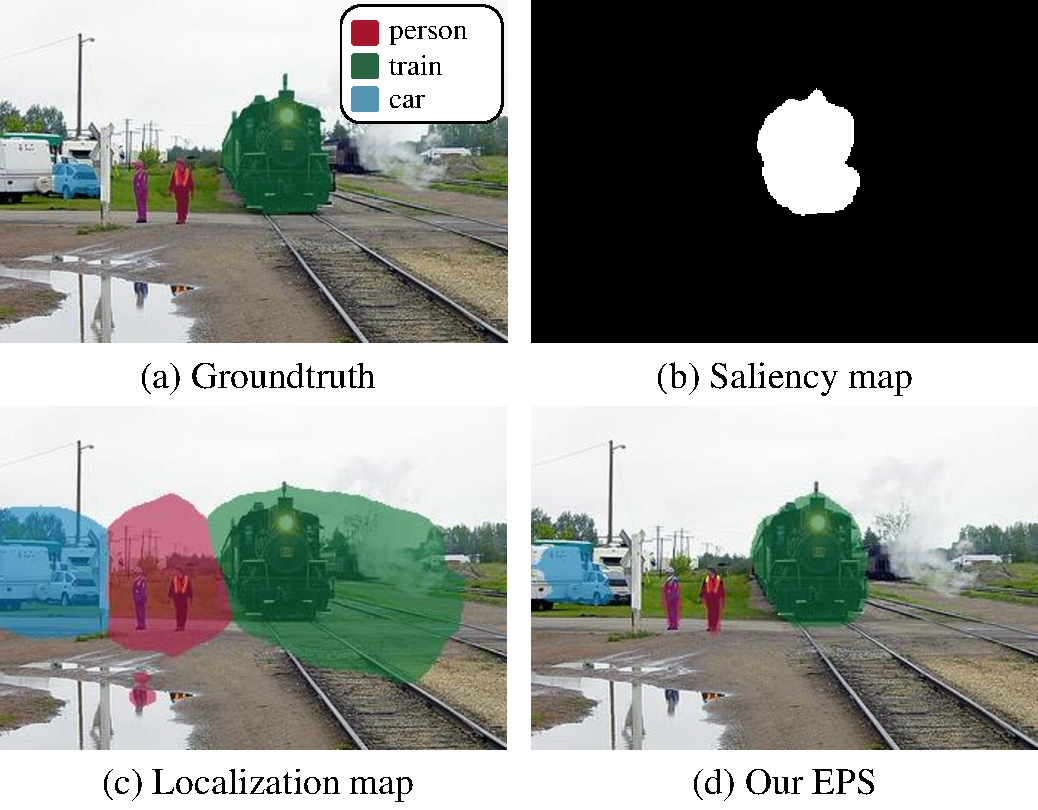
\includegraphics[width=8 cm]{figures/fig_concept.pdf}
\caption{Motivating example of utilizing both the saliency map and the localization map for WSSS. (a) Groundtruth, (b) saliency map via PFAN~\cite{zhao2019pyramid}, (c) localization map via CAM~\cite{zhou2016learning} and (d) our EPS utilizing both the saliency map and the localization map for training a classifier. Note that the saliency map cannot capture \emph{person} and \emph{car} while our result can correctly restore them, and the localization map overly captures two objects.} \vspace{-2mm}
\label{fig:concept}
\end{figure}

이 문제를 해결하기 위해 기존 연구들은 세 가지 기둥으로 분류될 수 있습니다. 첫 번째 접근법은 픽셀을 지우거나~\cite{choe2020attention,kim2017two, li2018tell}, 점수 맵을 앙상블하거나~\cite{jiang2019integral, lee2019ficklenet}, 자가 지도 신호를 사용하여~\cite{wang2020self} 객체의 전체 범위를 포착하기 위해 객체 커버리지를 확장합니다. 그러나 이들은 객체의 형태를 안내할 단서가 없기 때문에 대상 객체의 정확한 경계를 결정하지 못합니다. 두 번째 접근법은 의사 마스크의 객체 경계를 개선하는 데 중점을 둡니다~\cite{fan2020learning,chen2020boundary}. 이들은 효과적으로 객체 경계를 학습하기 때문에 자연스럽게 경계까지 의사 마스크를 확장합니다. 그러나 여전히 비대상 객체의 일치하는 픽셀을 대상 객체와 구별하지 못합니다. 이는 전경과 배경 간의 강한 상관관계(즉, 동시 발생)가 유도 편향(즉, 대상 객체와 그 일치하는 픽셀을 관찰하는 빈도)과 거의 구별되지 않기 때문입니다~\cite{choe2020evaluating}. 마지막으로, 세 번째 접근법은 추가적인 실제 마스크~\cite{BMVC2016_92} 또는 주목도 맵~\cite{oh2017exploiting, yao2020saliency}을 사용하여 동시 발생 문제를 완화하는 것을 목표로 합니다. 그러나 \cite{BMVC2016_92,li2018tell}은 약한 지도 학습 패러다임과는 거리가 먼 강력한 픽셀 수준 주석이 필요합니다. \cite{oh2017exploiting}은 주목도 맵의 오류에 민감합니다. 또한 \cite{yao2020saliency}는 객체의 전체 범위를 다루지 않으며 경계 불일치로 고통받습니다.

이 논문에서 우리의 목표는 이미지 수준 레이블로 학습된 이미지 분류기에서의 CAM(즉, CAM)과 기성품 주목도 탐지 모델의 출력(즉, 주목도 맵) 모두를 완전히 활용하여 WSSS의 세 가지 과제를 극복하는 것입니다~\cite{hou2017deeply,nguyen2019deepusps,zhao2019pyramid}. 우리는 위치 맵과 주목도 맵의 상호 보완적 관계에 중점을 둡니다. 그림~\ref{fig:concept}에 설명된 바와 같이, 위치 맵은 서로 다른 객체를 구별할 수 있지만 그들의 경계를 효과적으로 분리하지는 못합니다. 반대로, 주목도 맵은 풍부한 경계 정보를 제공하지만 객체의 정체성을 드러내지 않습니다. 이러한 의미에서, 우리는 두 가지 상호 보완적인 정보를 사용하는 우리의 방법이 WSSS의 성능 병목을 해결할 수 있다고 주장합니다.

이를 위해, 우리는 WSSS를 위한 새로운 프레임워크인 \emph{명시적 의사-픽셀 감독(EPS)}을 제안합니다. 주목도 맵(즉, 전경과 배경 모두)을 완전히 활용하기 위해, 우리는 $C$ 대상 클래스와 배경 클래스로 구성된 $C+1$ 클래스를 예측하기 위한 분류기를 설계합니다. 우리는 $C$ 위치 맵과 배경 위치 맵을 활용하여 주목도 맵을 추정합니다. 그런 다음, 주목도 손실은 주목도 맵과 우리의 추정된 주목도 맵 간의 픽셀 단위 차이로 정의됩니다. 주목도 손실을 도입함으로써, 모델은 모든 클래스에 걸쳐 의사-픽셀 피드백에 의해 감독될 수 있습니다. 우리는 또한 이미지 수준 레이블을 예측하기 위해 다중 레이블 분류 손실을 사용합니다. 따라서, 우리는 분류기를 주목도 손실과 다중 레이블 분류 손실을 최적화하도록 훈련하여 배경과 전경 픽셀 모두에 대한 예측을 시너지화합니다. 우리의 전략이 주목도 맵(섹션~\ref{section3.3} 및 그림~\ref{fig:sal})과 의사 마스크(섹션~\ref{section:5.1} 및 그림~\ref{fig:ablation}) 모두를 개선할 수 있음을 발견했습니다.

우리는 주목도 손실이 의사-픽셀 피드백을 통해 경계 불일치를 벌하기 때문에, 우리의 방법이 객체의 정확한 경계를 학습하도록 강제할 수 있음을 강조합니다. 부수적으로, 우리는 경계까지 맵을 확장하여 전체 객체를 포착할 수도 있습니다. 주목도 손실이 전경(예: 기차)과 배경을 분리하는 데 도움을 주기 때문에, 우리의 방법은 동시 발생하는 픽셀(예: 철도)을 배경 클래스로 할당할 수 있습니다. 실험 결과는 우리의 EPS가 PASCAL VOC 2012 및 MS COCO 2014 데이터셋에서 새로운 최첨단 정확도를 기록하며 놀라운 세분화 성능을 달성했음을 보여줍니다.

\section{관련 연구}

\noindent\textbf{약한 지도 학습 기반 의미론적 세분화.}
WSSS의 일반적인 파이프라인은 분류 네트워크에서 의사 마스크를 생성하고, 이 의사 마스크를 감독으로 사용하여 세그멘테이션 네트워크를 훈련하는 것입니다. 이미지 수준 레이블에서 경계 정보가 부족하기 때문에 많은 기존 방법들은 부정확한 의사 마스크로 고통받습니다. 이 문제를 해결하기 위해, 교차 이미지 친화성~\cite{fan2020cian}, 지식 그래프~\cite{liu2020leveraging}, 대조 최적화~\cite{sun2020mining, zhang2020splitting} 등이 의사 마스크의 품질을 향상시키기 위해 사용됩니다. \cite{chang2020weakly}는 CAM을 개선하기 위해 분류기를 강화하는 하위 카테고리를 발견하는 자기 지도 학습 과제를 제안합니다. \cite{ahn2019weakly, ahn2018learning}은 픽셀 간의 친화성을 계산하여 경계 정보를 암묵적으로 활용합니다. \cite{zhang2020reliability}는 신뢰할 수 있는 픽셀 수준 주석을 생성하는 데 중점을 두고 세그멘테이션 맵을 생성하기 위한 종단 간 네트워크를 설계합니다. \cite{huang2018weakly, kolesnikov2016seed}는 경계 손실을 활용하여 세그멘테이션 네트워크를 훈련합니다. 최근 \cite{araslanov2020single}는 자기 지도 학습 체계를 가진 단일 세그멘테이션 기반 모델을 사용합니다. \cite{fan2020employing}은 여러 불완전한 의사 마스크를 활용하여 세그멘테이션 네트워크의 견고성에 중점을 둡니다.

\begin{figure*}[t]
\centering
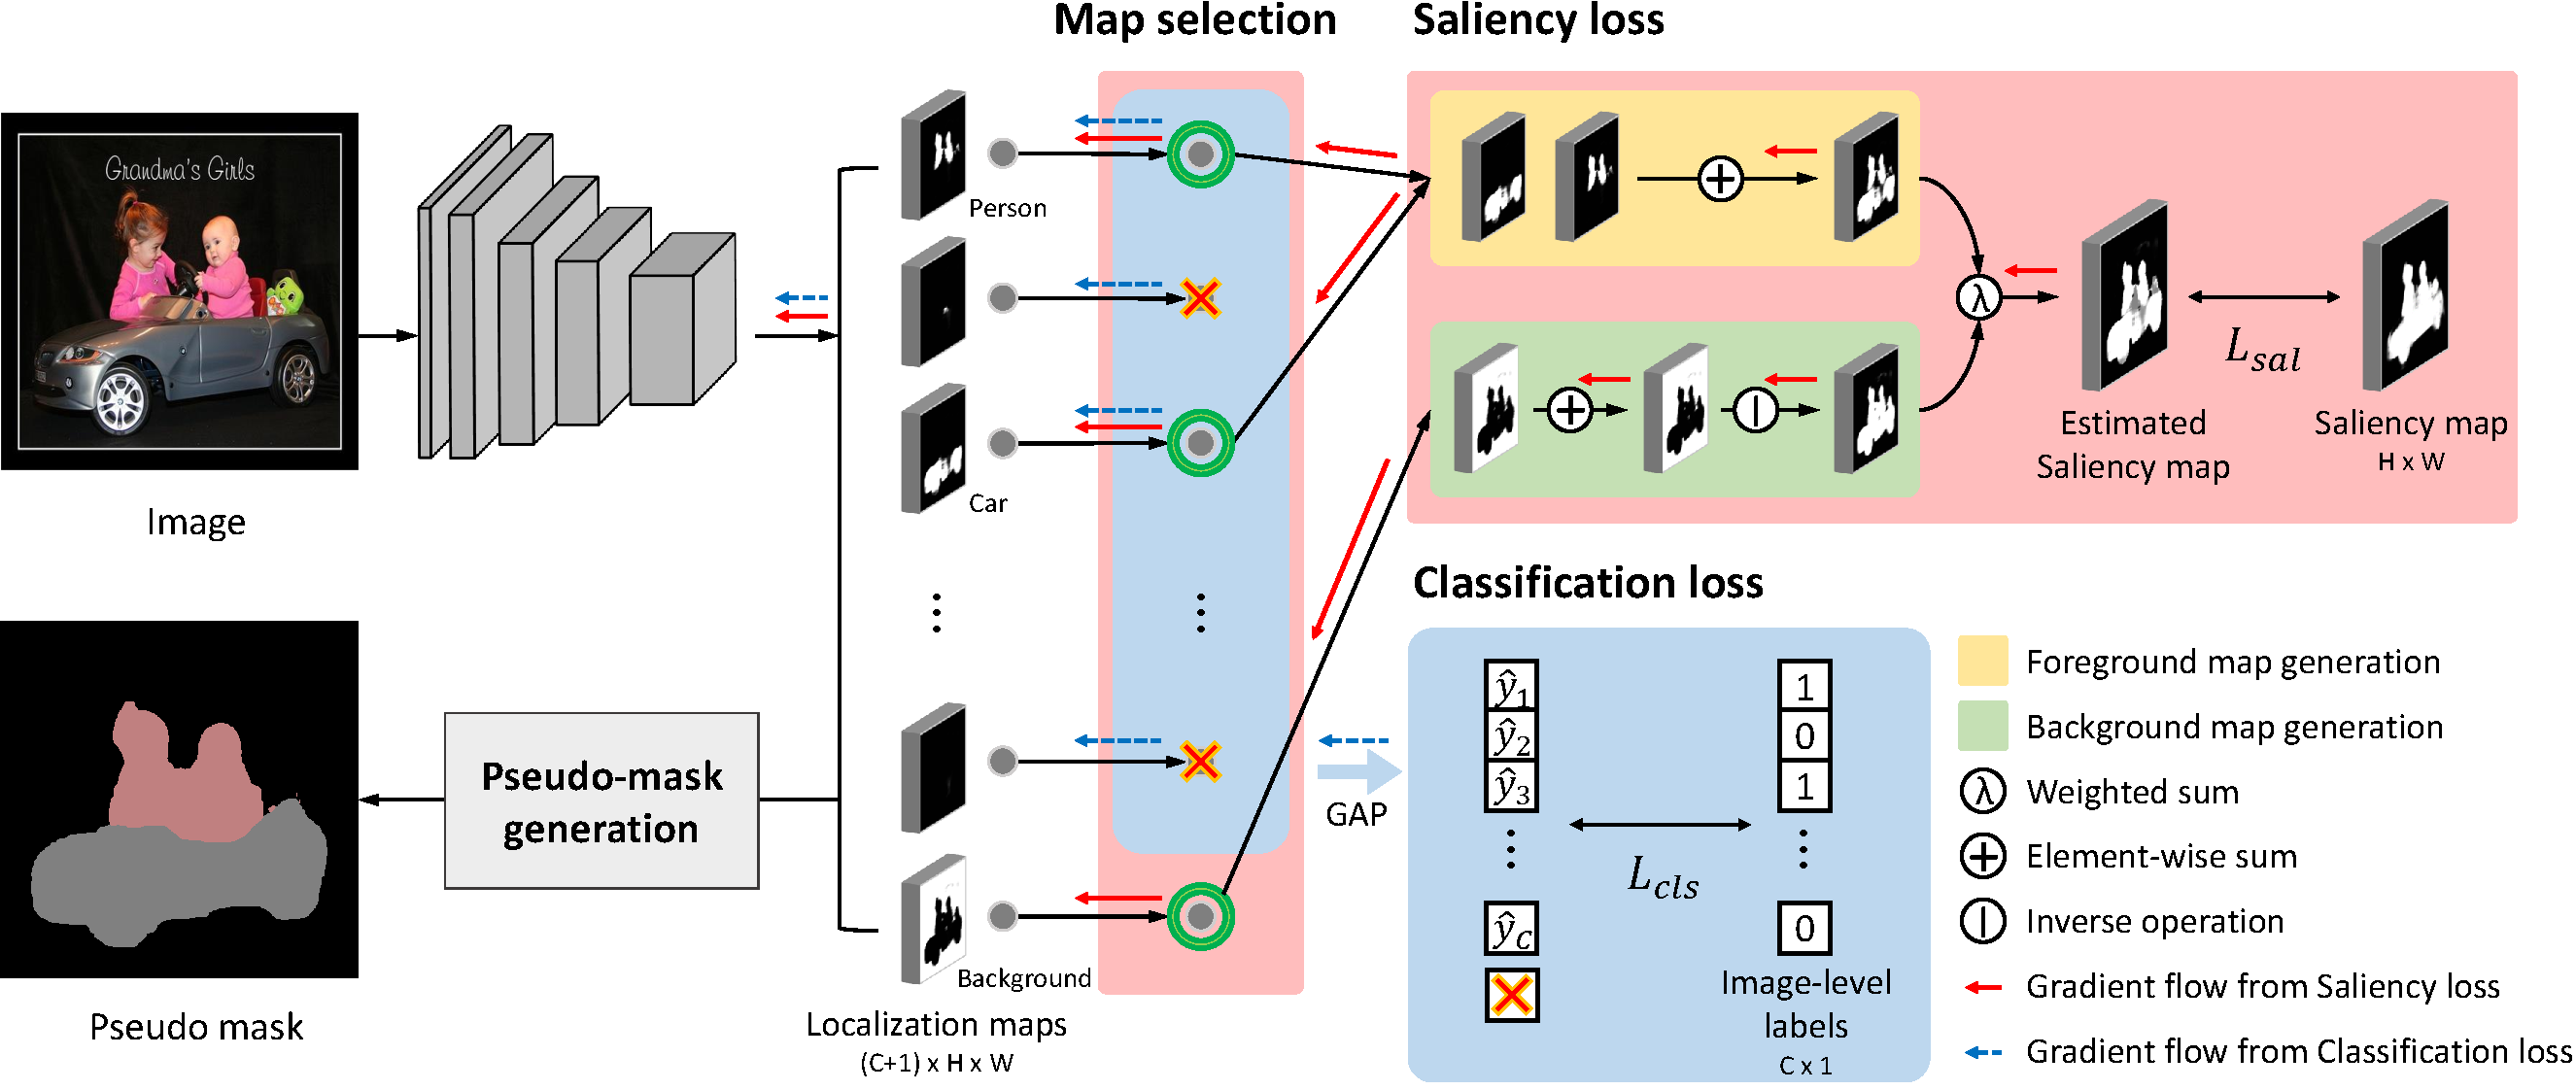
\includegraphics[width=16cm]{figures/framework.pdf}
\caption{我々のEPSの全体的なフレームワーク。$C+1$のローカライゼーションマップがバックボーンネットワークから生成されます。実際の顕著性マップは、既製の顕著性検出モデルから生成されます。ターゲットラベルのためのいくつかのローカライゼーションマップは、推定顕著性マップを生成するために選択的に使用されます(セクション~\ref{section3.2})。全体的なフレームワークは、顕著性損失と分類損失と共に共同で訓練されます(セクション~\ref{section3.3})。} \vspace{-2mm}
\label{fig:framework}
\end{figure*}


\vspace{1mm}
\noindent\textbf{주목성 유도 의미론적 세그멘테이션.}
주목성 탐지(SD) 방법은 픽셀 수준 주석~\cite{hou2017deeply, xiao2018deep, zhao2019pyramid} 또는 이미지 수준 주석~\cite{wang2017learning}이 있는 외부 주목성 데이터셋을 통해 이미지에서 전경과 배경을 구별하는 주목성 맵을 생성합니다. 많은 WSSS 방법들~\cite{fan2020cian, huang2018weakly, lee2019ficklenet, li2018tell, wei2017object, wei2018revisiting}은 의사 마스크의 배경 단서로 주목성 맵을 활용합니다. \cite{wei2016stc}는 단일 객체 이미지의 완전한 감독으로 주목성 맵을 활용합니다. \cite{fan2018associating}은 객체의 유사성 그래프를 학습하기 위해 인스턴스 수준 주목성 맵을 사용합니다. \cite{chaudhry_dcsp_2017, wang2018weakly, yao2020saliency}는 클래스별 주의 단서와 주목성 맵을 결합하여 신뢰할 수 있는 의사 마스크를 생성합니다. \cite{zeng2019joint}은 단일 네트워크를 사용하여 WSSS와 SD를 공동으로 해결하여 두 작업의 성능을 향상시킵니다. 우리의 EPS는 주목성 유도 방법으로 분류될 수 있지만 다음과 같은 이유로 다른 모든 방법과 명확히 구별됩니다. 대부분의 기존 방법은 의사 마스크의 일부로 또는 분류기의 중간 특징을 정제하기 위한 암묵적 지침으로 주목성 맵을 활용합니다. 반대로, 우리의 방법은 주목성 맵을 로컬라이제이션 맵에 대한 의사 픽셀 피드백으로 활용합니다. \cite{zeng2019joint}은 두 가지 보완 정보를 활용하는 점에서 우리와 가장 유사한 작업이지만, 그들은 공존 문제를 해결하지 않거나 노이즈가 있는 주목성 맵 문제를 처리하지 않습니다.

\section{제안된 방법}

이 섹션에서는 \emph{명시적 의사 픽셀 감독(EPS)}이라고 불리는 약한 감독 의미론적 세그멘테이션(WSSS)을 위한 새로운 프레임워크를 제안합니다. WSSS의 두 단계를 고려할 때, 첫 번째 단계는 의사 마스크를 생성하고 두 번째 단계는 세그멘테이션 모델을 훈련하는 것입니다. 여기서 우리의 주요 기여는 정확한 의사 마스크를 생성하는 것입니다. WSSS 관례를 따르며~\cite{fan2020learning,jiang2019integral,lee2019ficklenet,li2018tell,wang2020self,wei2017object}, 우리는 첫 번째 단계에서 생성된 의사 마스크를 감독으로 사용하여 세그멘테이션 모델을 훈련합니다.

\subsection{동기}
\label{section3.1}

EPS의 핵심 통찰력은 두 가지 보완 정보를 완전히 활용하는 것입니다, 즉, 로컬라이제이션 맵에서의 객체 정체성과 주목성 맵에서의 경계 정보입니다. 이를 위해, 우리는 주목성 맵을 대상 레이블과 배경 모두에 대한 로컬라이제이션 맵에 대한 의사 픽셀 피드백으로 활용합니다. 우리는 추가적인 배경 클래스를 가진 분류기를 고안하여 총 $C+1$ 클래스를 예측하도록 하며, 이는 그림~\ref{fig:framework}에 나타나 있습니다. 이 분류기를 사용하여, 우리는 $C+1$ 로컬라이제이션 맵을 학습할 수 있습니다, 즉, 대상 레이블에 대한 $C$ 로컬라이제이션 맵과 배경 로컬라이제이션 맵입니다.
우리는 EPS가 WSSS에서 경계 불일치 문제와 동시 발생 문제를 어떻게 해결할 수 있는지 설명합니다. 경계 불일치 문제를 관리하기 위해, 우리는 $C$ 지역화 맵에서 전경 맵을 추정하고 이를 주목도 맵의 전경과 일치시킵니다. 이렇게 하면, 대상 레이블의 지역화 맵이 주목도 맵으로부터 의사-픽셀 피드백을 받아 객체의 경계를 개선할 수 있습니다. 비대상 객체의 동시 발생 픽셀을 완화하기 위해, 우리는 배경에 대한 지역화 맵도 주목도 맵과 일치시킵니다. 배경에 대한 지역화 맵도 주목도 맵으로부터 의사-픽셀 피드백을 받기 때문에, 동시 발생 픽셀은 성공적으로 배경에 할당될 수 있습니다; 비대상 객체의 동시 발생 픽셀은 대부분 배경과 겹칩니다. 이것이 우리의 방법이 대상 객체로부터 동시 발생 픽셀을 분리할 수 있는 이유입니다.
\begin{figure}[t]
\centering
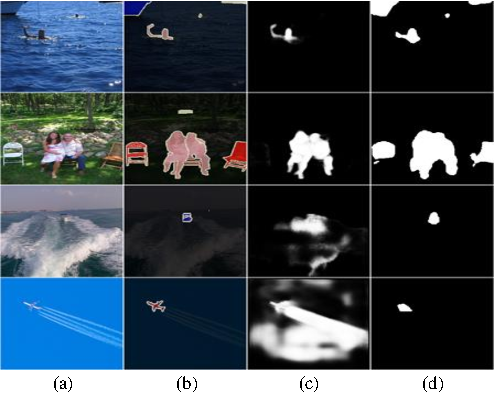
\includegraphics[width=8cm]{figures/fig_saliency_v2.pdf}
\caption{在 PASCAL VOC 2012 上估計的顯著性圖的質性範例。(a) 輸入圖像,(b) 真實值,(c) 來自 \cite{zhao2019pyramid} 的顯著性圖和 (d) 我們估計的顯著性圖。} \vspace{-2mm}
\label{fig:sal}
\end{figure}

마지막으로, EPS의 목적 함수는 두 부분으로 구성됩니다: {주목도 손실} $\mathcal{L}_{sal}$ (그림~\ref{fig:framework}의 빨간 상자/화살표로 표시됨)과 이미지 수준 레이블을 통한 {다중 레이블 분류 손실} $\mathcal{L}_{cls}$ (그림~\ref{fig:framework}의 파란 상자/화살표로 표시됨)입니다. 두 목표를 공동으로 훈련함으로써, 우리는 보완적인 정보로 지역화 맵과 주목도 맵을 시너지화할 수 있습니다-- 우리는 그림~\ref{fig:sal}에서 설명된 바와 같이, 서로의 노이즈와 누락된 정보가 우리의 공동 훈련 전략을 통해 보완된다는 것을 관찰합니다. 예를 들어, 기성 모델~\cite{hou2017deeply,nguyen2019deepusps,zhao2019pyramid}에서 얻은 원래의 주목도 맵은 누락된 정보와 노이즈가 있습니다. 반면에, 우리의 결과는 누락된 객체(예: 보트나 의자)를 성공적으로 복원하고 노이즈(예: 물방울이나 비행운)를 제거하여 원래의 주목도 맵보다 명백히 더 나은 결과를 보여줍니다. 결과적으로, EPS는 더 정확한 객체 경계를 포착하고 대상 객체로부터 동시 발생 픽셀을 분리할 수 있습니다. 이러한 장점은 놀라운 성능 향상을 가져옵니다; 표~\ref{tab:seg_quan_voc_resnet101}은 EPS가 기존 모델을 최대 3.8--10.6%의 세분화 정확도 향상으로 놀랍게 능가한다는 것을 보고합니다.

\subsection{명시적 의사-픽셀 감독}\label{section3.2}

우리는 의사-픽셀 감독을 위해 주목도 맵을 어떻게 활용할 수 있는지 설명합니다. 주목도 맵의 주요 장점은 객체의 실루엣을 제공하여 객체 경계를 더 잘 드러낼 수 있다는 것입니다. 이 속성을 활용하기 위해, 우리는 주목도 맵을 전경과 배경 두 가지 경우와 일치시킵니다. 클래스별 지역화 맵을 주목도 맵과 비교 가능하게 만들기 위해, 우리는 대상 레이블의 지역화 맵을 병합하고 전경 맵 $\mathbf{M}_{fg} \in \mathbb{R}^{H \times W}$을 생성합니다. 우리는 또한 배경 레이블에 대한 지역화 맵인 배경 맵 $\mathbf{M}_{bg} \in \mathbb{R}^{H \times W}$의 반전을 수행하여 전경을 나타낼 수 있습니다. (나중에, 우리는 노이즈가 있는 주목도 맵을 해결하기 위해 전경 맵을 어떻게 정제하는지 설명합니다.)

구체적으로, 우리는 다음과 같이 $\mathbf{M}_{fg}$와 $\mathbf{M}_{bg}$를 사용하여 주목도 맵 $\mathbf{\hat{M}}_{s}$를 추정합니다:\vspace{-1mm}
\begin{equation}
\label{eq_esimate_sal}
{\small
\begin{split}
\mathbf{\hat{M}}_{s} = \lambda\mathbf{M}_{fg} + (1-\lambda)(1-\mathbf{M}_{bg}),
\end{split}}\vspace{-1mm}
\end{equation}
\noindent 여기서 $\lambda \in [0, 1]$은 전경 맵과 배경 맵의 반전의 가중 합을 조정하는 하이퍼파라미터입니다. (기본적으로, 우리는 실험에서 $\lambda$를 0.5로 설정하고 $\lambda$에 대한 추가적인 소거 연구는 보충 자료에서 찾을 수 있습니다.) 그런 다음, 우리는 추정된 주목도 맵과 실제 주목도 맵 간의 픽셀별 차이의 합으로 주목도 손실 $\mathcal{L}_{sal}$을 정의합니다. (\ref{section3.3}에서 $\mathcal{L}_{sal}$의 공식 정의가 제시됩니다.)

사전 훈련된 모델을 사용하는 것은 약한 감독 학습으로 간주되며, 따라서 주목도 맵을 활용하는 것은 WSSS에서 일반적인 관행으로 널리 받아들여졌습니다. 그 인기에 불구하고, 완전 감독 주목도 탐지 모델을 채택하는 것은 다른 데이터셋에서 픽셀 수준 주석을 사용하기 때문에 논란의 여지가 있을 수 있습니다. 이 논문에서는 다양한 주목도 탐지 방법의 효과를 조사합니다; 1) 비지도 및 2) 완전 감독 주목도 탐지 모델 (\ref{section5.3} 참조), 그리고 경험적으로 우리의 방법이 그 중 어느 것을 사용하더라도 모든 다른 방법~\cite{fan2020learning,jiang2019integral,wang2018weakly, wei2016stc,yao2020saliency}을 능가한다는 것을 보여줍니다. 기존 방법이 주목도 맵을 완전히 활용하는 데 제한이 있는 반면, 우리의 방법은 주목도 맵을 의사-픽셀 감독으로 통합하고 경계와 동시 발생 픽셀에 대한 단서로 활용합니다.

\vspace{1mm}
\noindent\textbf{살리언시 편향을 처리하기 위한 맵 선택.} 이전에는 전경 맵이 타겟 레이블의 로컬라이제이션 맵의 합집합이 될 수 있다고 가정했습니다. 배경 맵은 배경 레이블의 로컬라이제이션 맵이 될 수 있습니다. 그러나 이러한 단순한 선택 규칙은 기성 모델에 의해 계산된 살리언시 맵과 호환되지 않을 수 있습니다. 예를 들어, \cite{zhao2019pyramid}의 살리언시 맵은 종종 일부 객체를 살리언트 객체로 무시합니다(예: 그림~\ref{fig:concept}의 기차 근처의 작은 사람들). 이러한 체계적인 오류는 살리언시 모델이 다양한 데이터셋의 통계를 학습하기 때문에 불가피합니다. 이 오류를 고려하지 않으면 동일한 오류가 우리 모델에 전파되어 성능 저하를 초래할 수 있습니다.

체계적인 오류를 해결하기 위해, 우리는 로컬라이제이션 맵과 살리언시 맵 간의 중첩 비율을 사용하는 효과적인 전략을 개발했습니다. 구체적으로, $i$번째 로컬라이제이션 맵 $\mathbf{M}_{i}$는 살리언시 맵과 $\tau$\% 이상 중첩되면 전경에 할당되고, 그렇지 않으면 배경에 할당됩니다. 공식적으로, 전경과 배경 맵은 다음과 같이 계산됩니다: \vspace{-1mm}
\begin{equation}
\label{eq_map_selection}
{\small
\begin{split}
&\mathbf{M}_{fg} = \sum_{i=1}^{C} {y_{i} \cdot \mathbf{M}_{i} \cdot \mathbbm{1}[\mathcal{O}(\mathbf{M}_i, \mathbf{M}_{s}) > \tau]}, \\
&\mathbf{M}_{bg} = \sum_{i=1}^{C} {y_{i} \cdot \mathbf{M}_{i} \cdot \mathbbm{1}[\mathcal{O}(\mathbf{M}_i, \mathbf{M}_{s}) \le \tau]} + \mathbf{M}_{C+1},
\end{split}}\vspace{-1mm}
\end{equation}
\noindent 여기서 $y \in \mathbb{R}^C$는 이진 이미지 레벨 레이블이고 $\mathcal{O}(\mathbf{M}_i, \mathbf{M}_{s})$는 $\mathbf{M}_i$와 $\mathbf{M}_{s}$ 간의 중첩 비율을 계산하는 함수입니다. 이를 위해, 우리는 먼저 로컬라이제이션 맵과 살리언시 맵을 이진화합니다: 픽셀 p에 대해, $\mathbf{B}_{k}(p) = 1$이면 $\mathbf{M}_{k}(p) > 0.5$; 그렇지 않으면 $\mathbf{B}_{k}(p) = 0$. $\mathbf{B}_{i}$와 $\mathbf{B}_{s}$는 각각 $\mathbf{M}_i$와 $\mathbf{M}_{s}$에 해당하는 이진화된 맵입니다. 그런 다음 $\mathbf{M}_i$와 $\mathbf{M}_{s}$ 간의 중첩 비율을 계산합니다, 즉, $\mathcal{O}(\mathbf{M}_i ,\mathbf{M}_{s}) = |\mathbf{B}_i \cap \mathbf{B}_{s}| / |\mathbf{B}_{i}|$. 우리는 데이터셋과 백본 모델에 관계없이 $\tau=0.4$로 설정합니다. 보충 자료에서, 우리는 $\tau$의 선택에 대해 우리의 방법이 강력하다는 것을 보여줍니다(즉, $\tau$가 [0.3, 0.5] 내에서 유사한 성능을 보입니다).

배경 레이블에 대한 단일 로컬라이제이션 맵 대신, 우리는 배경 레이블에 대한 로컬라이제이션 맵을 전경으로 선택되지 않은 로컬라이제이션 맵과 결합합니다. 비록 간단하지만, 우리는 살리언시 맵의 오류를 우회하고 살리언시 맵에서 무시된 일부 객체를 효과적으로 학습할 수 있습니다. (표~\ref{tab:strategy}에서, 우리는 살리언시 맵의 오류를 극복하기 위한 제안된 전략의 효과를 보고합니다.)

\subsection{공동 학습 절차}\label{section3.3}

살리언시 맵과 이미지 레벨 레이블을 사용하여, EPS의 전체 학습 목표는 살리언시 손실 $\mathcal{L}_{sal}$과 분류 손실 $\mathcal{L}_{cls}$의 두 부분으로 구성됩니다. 먼저, 살리언시 손실 $\mathcal{L}_{sal}$은 실제 살리언시 맵 $\mathbf{M}_{s}$와 추정된 살리언시 맵 $\mathbf{\hat{M}}_{s}$ 간의 평균 픽셀 레벨 거리를 측정하여 공식화됩니다.\vspace{-1mm}
\begin{equation}
{\small
\label{loss_sal}
\mathcal{L}_{sal} = \frac{1}{H\cdot W}||\mathbf{M}_{s}-\mathbf{\hat{M}}_{s}||^{2},
}\vspace{-1mm}
\end{equation}
\noindent 여기서 $\mathbf{M}_{s}$는 DUTS 데이터셋~\cite{wang2017learning}에서 훈련된 기성 살리언시 탐지 모델-- PFAN~\cite{zhao2019pyramid}에서 얻은 것입니다. 우리의 방법은 살리언시 탐지 모델에 관계없이 모든 이전 예술을 일관되게 능가합니다.

다음으로, 분류 손실은 각 타겟 클래스에 대한 로컬라이제이션 맵에 대한 글로벌 평균 풀링의 결과인 이미지 레벨 레이블 $y$와 그 예측 $\hat{y} \in \mathbb{R}^C$ 간의 다중 레이블 소프트 마진 손실로 계산됩니다.\vspace{-1mm}
\begin{equation}
{\small
\begin{split}
\label{loss_cls}
\mathcal{L}_{cls}= - \frac{1}{C} \sum_{i=1}^{C} y_i \log{\sigma(\hat{y_i})} + (1-y_i) \log{(1 - \sigma(\hat{y_i}))},
\end{split}}\vspace{-1mm}
\end{equation}
\noindent 여기서 $\sigma(\cdot)$는 시그모이드 함수입니다. 마지막으로, 총 학습 손실은 다중 레이블 분류 손실과 살리언시 손실의 합입니다, 즉, $\mathcal{L}_{total} = \mathcal{L}_{cls} + \mathcal{L}_{sal}$. 

그림~\ref{fig:framework}에서 보이는 것처럼, $\mathcal{L}_{sal}$은 대상 객체와 배경을 포함한 $C+1$ 클래스의 매개변수를 업데이트하는 데 관여합니다. 반면, $\mathcal{L}_{cls}$는 배경 클래스를 제외한 $C$ 클래스의 레이블 예측만 평가하며, $\mathcal{L}_{cls}$의 그래디언트는 배경 클래스로 흐르지 않습니다. 그러나, $\mathcal{L}_{cls}$는 분류기 훈련을 감독하기 때문에 배경 클래스의 예측에 암묵적으로 영향을 미칠 수 있습니다.

\section{실험 설정}
\noindent
\textbf{데이터셋}. 우리는 두 개의 인기 있는 벤치마크 데이터셋, PASCAL VOC 2012~\cite{everingham2015pascal}와 MS COCO 2014~\cite{lin2014microsoft}에 대한 실증 연구를 수행합니다. PASCAL VOC 2012는 21개의 클래스(즉, 20개의 객체와 배경)로 구성되어 있으며, 각각 1,464, 1,449, 1,456개의 훈련, 검증, 테스트 세트 이미지를 포함합니다. 의미론적 분할의 일반적인 관행에 따라, 우리는 10,582개의 이미지로 구성된 증강된 훈련 세트를 사용합니다~\cite{hariharan2011semantic}. 다음으로, COCO 2014는 배경을 포함한 81개의 클래스로 구성되어 있으며, 훈련과 검증을 위해 각각 82,081개와 40,137개의 이미지를 포함하고 있으며, 대상 클래스가 없는 이미지는~\cite{choe2020attention}에서와 같이 제외됩니다. 일부 객체의 실제 분할 레이블이 서로 겹치기 때문에, 우리는 동일한 COCO 데이터셋에서 겹침 문제를 해결한 COCO-Stuff~\cite{caesar2018coco}의 실제 분할 레이블을 채택합니다.

\vspace{0.5mm}
\noindent
\textbf{평가 프로토콜}. 우리는 PASCAL VOC 2012의 검증 및 테스트 세트와 COCO 2014의 검증 세트로 우리의 방법을 검증합니다. PASCAL VOC 2012의 테스트 세트에 대한 평가 결과는 공식 PASCAL VOC 평가 서버에서 얻습니다. 또한, 우리는 분할 모델의 정확성을 측정하기 위해 평균 교차-오버-유니온(mIoU)을 채택합니다.

\vspace{0.5mm}
\noindent
\textbf{구현 세부사항}. 우리는 출력 스트라이드가 8인 ResNet38~\cite{wu2019wider}을 우리의 방법의 백본 네트워크로 선택합니다. 모든 백본 모델은 ImageNet~\cite{deng2009imagenet}에서 사전 훈련되었습니다. 우리는 배치 크기가 8인 SGD 옵티마이저를 사용합니다. 우리의 방법은 학습률 0.01(마지막 컨볼루션 레이어의 경우 0.1)로 20k 반복까지 훈련됩니다. 데이터 증강을 위해, 우리는 무작위 스케일링, 무작위 플리핑, 그리고 $448 \times 448$로 무작위 크롭을 사용합니다. 분할 네트워크의 경우, 우리는 DeepLab-LargeFOV (V1)~\cite{chen2014semantic}와 DeepLab-ASPP (V2)~\cite{chen2017deeplab}, 그리고 VGG16과 ResNet101을 백본 네트워크로 채택합니다. 구체적으로, 우리는 네 가지 분할 네트워크를 사용합니다: VGG16 기반 DeepLab-V1 및 DeepLab-V2, ResNet101 기반 DeepLab-V1 및 DeepLab-V2. 더 자세한 설정은 보충 자료에 있습니다.

\section{실험 결과}

\subsection{경계 및 동시 발생 처리}\label{section:5.1}

\noindent\textbf{경계 불일치 문제}. 의사 마스크의 경계를 검증하기 위해, 우리는 최신 방법~\cite{chen2020boundary, wang2020self, zhou2016learning}과 경계의 품질을 비교합니다. 우리는 PASCAL VOC 2011에서 경계 주석과 경계 벤치마크를 제공하는 SBD~\cite{hariharan2011semantic}를 활용합니다. ~\cite{chen2020boundary}에서와 같이, 경계의 품질은 라플라시안 에지 검출기로부터 의사 마스크의 에지를 계산하여 클래스 비특이적 방식으로 평가됩니다. 그런 다음, 예측된 경계와 실제 경계를 비교하여 재현율, 정밀도, F1-스코어를 측정하여 경계 품질을 평가합니다. 표~\ref{tab:boundary}는 우리의 방법이 모든 세 가지 메트릭에서 다른 방법보다 크게 우수하다는 것을 보고합니다. 그림~\ref{fig:ablation}의 정성적 예시는 우리의 방법이 다른 모든 방법보다 더 정확한 경계를 포착할 수 있음을 보여줍니다.

\begin{figure}[t]
\centering
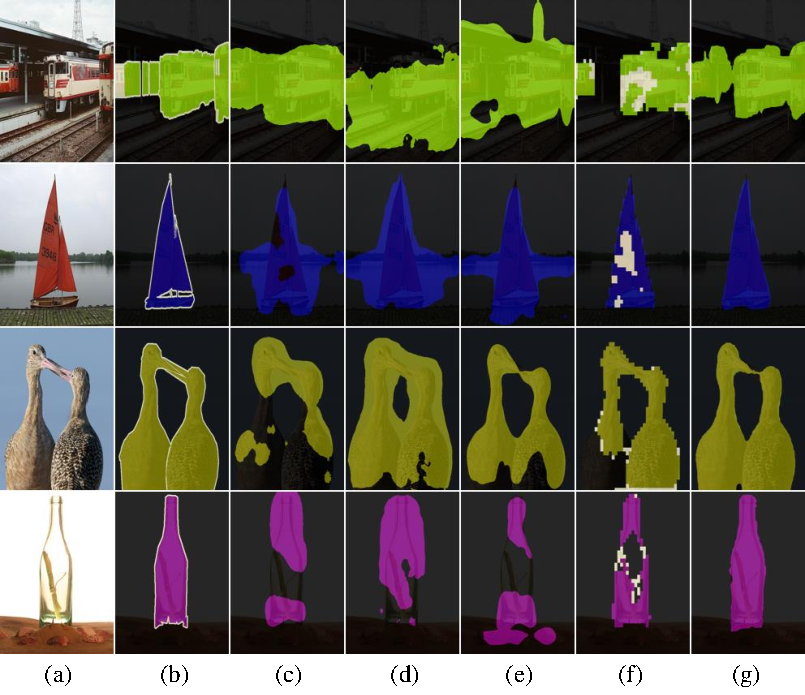
\includegraphics[width=8cm]{figures/fig_ablation.pdf}
\caption{Qualitative comparison for pseudo-masks on PASCAL VOC 2012. (a) Input images, (b) groundtruth, (c) CAM, (d) SEAM, (e) ICD, (f) SGAN and (g) our EPS.}
\label{fig:ablation} \vspace{-3mm}
\end{figure}


\begin{table}[]
\centering
{\small
\begin{tabular}{@{}lccc@{}}
\toprule
\multicolumn{1}{c}{方法}                      & 召回率(\%) & 精确率(\%) & F1-分数(\%) \\ \midrule
\multicolumn{1}{l}{CAM~\cite{zhou2016learning}\textsubscript{CVPR'16}} & 22.3        & 35.8           & 27.5           \\
\multicolumn{1}{l}{SEAM~\cite{wang2020self}\textsubscript{CVPR'20}}    & 40.2        & 45.0           & 42.5           \\
\multicolumn{1}{l}{BES~\cite{chen2020boundary}\textsubscript{ECCV'20}} & 45.5        & 46.4           & 45.9           \\
\multicolumn{1}{l}{我们的 EPS}                        & 60.0        & 73.1          & 65.9           \\ \bottomrule
\end{tabular}
}
\vspace{2mm}
\caption{在 SBD trainval 集上评估的边界准确性。请注意,BES 的结果是从~\cite{chen2020boundary}中提出的边界预测网络测量的。} \vspace{-2mm}
\label{tab:boundary}
\end{table}


\vspace{1mm}
\noindent \textbf{동시 발생 문제}. 여러 연구~\cite{huang2018weakly, kolesnikov2016seed, li2018tell, oh2017exploiting}에서 논의된 바와 같이, 우리는 PASCAL VOC 2012에서 일부 배경 클래스가 대상 객체와 자주 함께 나타나는 것을 관찰합니다. 우리는 PASCAL-CONTEXT 데이터셋~\cite{mottaghi2014role}을 사용하여 동시 발생 객체의 빈도를 정량적으로 분석합니다. 이 데이터셋은 전체 장면에 대한 픽셀 수준 주석을 제공합니다(예: ~\emph{물} 및 ~\emph{철도}). 우리는 세 가지 동시 발생 쌍을 선택합니다; \emph{보트}와 \emph{물}, \emph{기차}와 \emph{철도}, 그리고 \emph{기차}와 \emph{플랫폼}. 우리는 대상 클래스에 대한 IoU와 대상 클래스와 그 동시 발생 클래스 간의 \emph{혼동 비율}을 비교합니다. 혼동 비율은 동시 발생 클래스가 대상 클래스로 잘못 예측되는 정도를 측정합니다. 혼동 비율 $m_{k,c}$는 $m_{k,c} = FP_{k,c}/TP_{c}$로 계산되며, 여기서 ${FP_{k,c}}$는 동시 발생 클래스 $k$에 대해 대상 클래스 $c$로 잘못 분류된 픽셀 수이고, $TP_{c}$는 대상 클래스 $c$에 대한 진양성 픽셀 수입니다. 동시 발생 문제에 대한 더 자세한 분석은 보충 자료에 있습니다.


Table~\ref{tab:co_quantitative_v4}는 EPS가 다른 방법들보다 일관되게 낮은 혼동 비율을 보인다고 보고합니다. SGAN~\cite{yao2020saliency}은 우리와 매우 유사한 혼동 비율을 가지고 있지만, 우리 방법은 IoU 측면에서 목표 클래스를 훨씬 정확하게 포착합니다. 흥미롭게도, SEAM은 높은 혼동 비율을 보이며 CAM보다도 나쁩니다. 이는 SEAM~\cite{wang2020self}이 자기 지도 학습을 적용하여 목표 객체의 전체 범위를 커버하도록 학습하기 때문인데, 이는 목표 객체의 우연한 픽셀에 쉽게 속습니다. 반면에, CAM은 목표 객체의 가장 변별적인 영역만 포착하고 덜 변별적인 부분, 예를 들어 우연한 클래스는 커버하지 않습니다. 우리는 이 현상을 Figure~\ref{fig:ablation}에서도 관찰할 수 있습니다.

% 請將以下所需的套件添加到您的文件前言:
% \usepackage{booktabs}

\newcommand{\R}{\textcolor{red}}
\newcommand{\B}{\textcolor{blue}}

\begin{table}[]
\centering
{\small
\begin{tabular}{@{}llll@{}}
\toprule
\multicolumn{1}{c}{\multirow{2}{*}{方法}} & \multicolumn{1}{c}{~\emph{船} w/}   & \multicolumn{1}{c}{~\emph{火車} w/}  & \multicolumn{1}{c}{~\emph{火車} w/}  \\
& \multicolumn{1}{c}{~\emph{水}} & \multicolumn{1}{c}{~\emph{鐵路}}          & \multicolumn{1}{c}{~\emph{平台}}  \\ \midrule
\multicolumn{1}{l}{CAM~\cite{zhou2016learning}\textsubscript{CVPR'16}}              & \B{0.74} (33.1)   & \B{0.11} (52.9)   & \multicolumn{1}{l}{\B{0.09} (49.6)}   \\
\multicolumn{1}{l}{SEAM~\cite{wang2020self}\textsubscript{CVPR'20}}                 & \B{1.13} (30.7)   & \B{0.24} (48.6)   & \multicolumn{1}{l}{\B{0.20} (45.5)}   \\
\multicolumn{1}{l}{ICD~\cite{fan2020learning}\textsubscript{CVPR'20}}               & \B{0.47} (41.4)   & \B{0.11} (56.7)   & \multicolumn{1}{l}{\B{0.09} (49.2)}   \\
\multicolumn{1}{l}{SGAN~\cite{yao2020saliency}\textsubscript{ACCESS'20}}            & \B{0.10} (42.3)   & \B{0.02} (48.8)   & \multicolumn{1}{l}{\B{0.01} (36.3)}   \\
\multicolumn{1}{l}{我們的 EPS}                                                         & \B{0.10} (55.0)   & \B{0.02} (78.1)   & \multicolumn{1}{l}{\B{0.01} (73.0)}   \\ \bottomrule
\end{tabular}
}
\vspace{2mm}
\caption{與現有代表性方法處理共現問題的比較。每個條目是 {$m_{k,c}$} 在~\B{藍色}中(越低越好),括號中的 IoU(越高越好)。} \vspace{-2mm}
\label{tab:co_quantitative_v4}

\end{table}

\begin{table}[]
%\resizebox{\columnwidth}{!}{%
\centering

{\small
\begin{tabular}{@{}ccccc@{}}
\toprule
                            & 基线  & 简单   & 预定义   & 我们的自适应 \\ \midrule
\multicolumn{1}{l}{mIoU}    &66.1       & 66.5      & 67.9          & 69.4   \\ \bottomrule
\end{tabular}
}
\vspace{2mm}
\caption{地图选择策略的效果。使用不同地图选择策略的伪掩码的准确性在 PASCAL VOC 2012 训练集上进行评估。} \vspace{-2mm}
\label{tab:strategy}
\end{table}


\subsection{맵 선택 전략의 효과}
우리는 주목성 맵의 오류를 완화하기 위한 맵 선택 전략의 효과를 평가합니다. 우리는 맵 선택 모듈을 사용하지 않는 기본선과 세 가지 다른 맵 선택 전략을 비교합니다. 가장 단순한 전략으로, 전경 맵은 모든 객체 위치 맵의 합집합이며, 배경 맵은 배경 클래스의 위치 맵과 같습니다(즉, 단순 전략). 다음으로, 우리는 다음 예외를 제외하고 단순 전략을 따릅니다. 몇몇 사전 결정된 클래스(예: \emph{소파}, \emph{의자}, \emph{식탁})의 위치 맵은 배경 맵에 할당됩니다(즉, 사전 정의된 클래스 전략). 마지막으로, 제안된 선택 방법은 Section~\ref{section3.2}에서 설명한 대로 위치 맵과 주목성 맵 간의 중첩 비율을 활용합니다(즉, 우리의 적응형 전략).

\begin{figure*}[t]
\centering
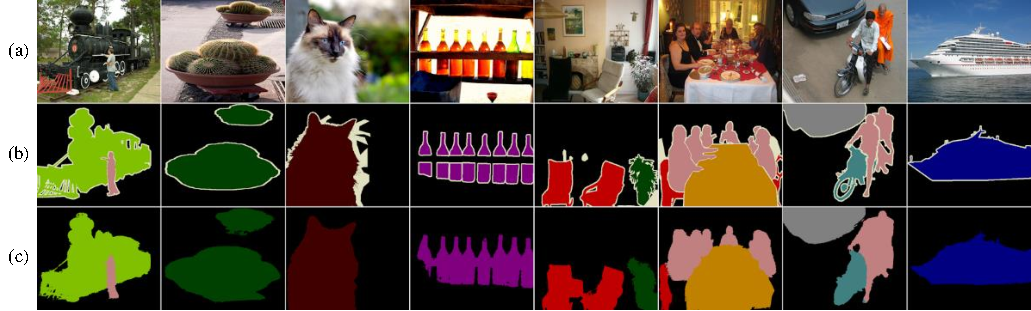
\includegraphics[width=17cm]{figures/segmentation_voc.pdf}
\caption{PASCAL VOC 2012 上分割结果的定性示例。(a) 输入图像,(b) 真实值和 (c) 我们的 EPS。}\vspace{-2mm}
\label{fig:seg_qual_voc}
\end{figure*}

\begin{table}[]
\centering
{\small
\begin{tabular}{@{}lccc@{}}
\toprule
\multicolumn{1}{c}{\multirow{2}{*}{Method}}         & w/o           & w/ &                                  w/ \\
                                                    & refinement    & CRF~\cite{krahenbuhl2011efficient}    & AffinityNet~\cite{ahn2018learning}    \\ \midrule
\multicolumn{1}{l}{CAM~\cite{zhou2016learning}\textsubscript{CVPR'16}}     & 48.0          & -                                     & 58.1                                  \\
\multicolumn{1}{l}{SEAM~\cite{wang2020self}\textsubscript{CVPR'20}}        & 55.4          & 56.8                                  & 63.6                                  \\
\multicolumn{1}{l}{ICD~\cite{chen2020boundary}\textsubscript{CVPR'20}*}     & 59.9          & 62.2                                  & -                                     \\
\multicolumn{1}{l}{SGAN~\cite{yao2020saliency}\textsubscript{ACCESS'20}*}     & 62.8          & -                                     & -                                     \\
\multicolumn{1}{l}{Our EPS}                            & 69.4          & 71.4                                  & 71.6                                  \\ \bottomrule
\end{tabular}
}
\vspace{2mm}
\caption{PASCAL VOC 2012のトレインセットで評価された擬似マスクの精度(mIoU)。*は低信頼度のピクセルが無視されることを示します。他の方法はすべてのピクセルを評価に使用します。} \vspace{-3mm}
\label{tab:refinement}
\end{table}


Table~\ref{tab:strategy}는 우리의 적응형 전략이 주목성 맵의 체계적인 편향을 효과적으로 처리할 수 있음을 보여줍니다. 단순 전략은 위치 맵에서 추정된 주목성 맵을 생성할 때 편향 고려가 없음을 의미합니다. 이 경우, 특히 \emph{소파}, \emph{의자} 또는 \emph{식탁} 클래스에서 의사 마스크의 성능이 저하됩니다. 사전 정의된 클래스를 사용하는 성능은 주목성 맵에서 누락된 클래스를 무시함으로써 편향을 완화할 수 있음을 보여줍니다. 그러나 이는 인간 관찰자에 의한 수동 선택이 필요하므로 덜 실용적이며 이미지별로 최적의 결정을 내릴 수 없습니다. 반면에, 우리의 적응형 전략은 편향을 자동으로 처리하고 주어진 주목성 맵에 대해 더 효과적인 결정을 내립니다.

\subsection{최신 기술과의 비교}
\label{section5.3}

\noindent \textbf{의사 마스크의 정확도.} 우리는~\cite{ahn2018learning,wang2020self}에서 사용된 일반적인 관행인 다양한 스케일의 이미지에서 예측 결과를 집계하여 다중 스케일 추론을 채택합니다. 그런 다음, 우리는 CAM~\cite{zhou2016learning}과 세 가지 최신 방법, 즉 SEAM~\cite{wang2020self}, ICD~\cite{fan2020learning}, SGAN~\cite{yao2020saliency}과 비교하여 학습 세트에서 의사 마스크의 정확도를 평가합니다. 여기서, 학습 세트에서 의사 마스크의 정확도를 측정하는 것은 WSSS에서 일반적인 프로토콜입니다. 왜냐하면 학습 세트의 의사 마스크가 세분화 모델을 감독하는 데 사용되기 때문입니다. Table~\ref{tab:refinement}은 의사 마스크의 정확도를 요약하고 우리의 방법이 기존의 모든 방법을 큰 차이로 능가함을 나타냅니다(즉, 7--21\% 차이). Figure~\ref{fig:ablation}은 의사 마스크의 질적 예를 시각화하여 우리의 방법이 객체 경계를 현저히 개선하고 의사 마스크의 품질 측면에서 세 가지 최신 방법을 크게 능가함을 확인합니다. 우리의 방법은 객체의 정확한 경계를 포착할 수 있으며(2번째 행) 따라서 객체의 전체 범위를 자연스럽게 커버하고(3번째 행) 우연한 픽셀을 완화할 수 있습니다(1번째 행). 우리의 방법의 더 많은 예제와 실패 사례는 보충 자료에 제공됩니다.

\begin{table}[]
\normalsize
\centering
{\small
\begin{tabular}{@{}lccll@{}}
\toprule
\multicolumn{1}{c}{방법}                                                              & 세그.      & 지원.  & \multicolumn{1}{c}{val} & \multicolumn{1}{c}{test} \\ \midrule
\multicolumn{1}{l}{SEC~\cite{kolesnikov2016seed}\textsubscript{ECCV'16}}                & V1        & I.    & 50.7                    & 51.7                     \\
\multicolumn{1}{l}{AffinityNet~\cite{ahn2018learning}\textsubscript{CVPR'18}}           & V1        & I.    & 58.4                    & 60.5                     \\
\multicolumn{1}{l}{ICD~\cite{fan2020learning}\textsubscript{CVPR'20}}                   & V1        & I.    & 61.2                    & 60.9                     \\
\multicolumn{1}{l}{BES~\cite{chen2020boundary}\textsubscript{ECCV'20}}                  & V1        & I.    & 60.1                    & 61.1                     \\
\multicolumn{1}{l}{GAIN~\cite{li2018tell}\textsubscript{CVPR'18}}                       & V1        & I.+S. & 55.3                    & 56.8                     \\
\multicolumn{1}{l}{MCOF~\cite{wang2018weakly}\textsubscript{CVPR'18}}                   & V1        & I.+S. & 56.2                    & 57.6                     \\
\multicolumn{1}{l}{SSNet~\cite{zeng2019joint}\textsubscript{ICCV'19}}                   & V1        & I.+S. & 57.1                    & 58.6                     \\
\multicolumn{1}{l}{DSRG~\cite{huang2018weakly}\textsubscript{CVPR'18}}                  & V2        & I.+S. & 59.0                    & 60.4                     \\
\multicolumn{1}{l}{SeeNet~\cite{hou2018self}\textsubscript{NeurIPS'18}}                 & V1        & I.+S. & 61.1                    & 60.7                     \\
\multicolumn{1}{l}{MDC~\cite{wei2018revisiting}\textsubscript{CVPR'18}}                 & V1        & I.+S. & 60.4                    & 60.8                     \\
\multicolumn{1}{l}{FickleNet~\cite{lee2019ficklenet}\textsubscript{CVPR'18}}            & V2        & I.+S. & 61.2                    & 61.9                     \\
\multicolumn{1}{l}{OAA~\cite{jiang2019integral}\textsubscript{ICCV'19}}                 & V1        & I.+S. & 63.1                    & 62.8                     \\
\multicolumn{1}{l}{ICD~\cite{fan2020learning}\textsubscript{CVPR'20}}                   & V1        & I.+S. & 64.0                    & 63.9                     \\
\multicolumn{1}{l}{Multi-Est.~\cite{fan2020employing}\textsubscript{ECCV'20}}           & V1        & I.+S. & 64.6                    & 64.2                     \\
\multicolumn{1}{l}{Split. \& Merge.~\cite{zhang2020splitting}\textsubscript{ECCV'20}}   & V2        & I.+S. & 63.7                    & 64.5                     \\
\multicolumn{1}{l}{SGAN~\cite{yao2020saliency}\textsubscript{ACCESS'20}}                & V2        & I.+S. & 64.2                    & 65.0                     \\ \midrule
\multicolumn{1}{l}{\multirow{2}{*}{우리의 EPS}}                                            & V1        & I.+S. & 66.6                    & \textbf{67.9}            \\
\multicolumn{1}{l}{}                                                                    & V2        & I.+S. & \textbf{67.0}           & 67.3                     \\ \bottomrule

\end{tabular}
}
\vspace{2mm}
\caption{PASCAL VOC 2012에서의 세그멘테이션 결과 (mIoU). 모든 결과는 VGG16을 기반으로 합니다. 모든 실험에서 최고의 점수는 굵게 표시되어 있습니다.}\vspace{-3mm}
\label{tab:seg_quan_voc_vgg16}
\end{table}

\begin{table}[]
\normalsize
\centering
{\small
\begin{tabular}{@{}lccll@{}}
\toprule
\multicolumn{1}{c}{Method}                                                              & Seg.      & Sup.  & \multicolumn{1}{c}{val} & \multicolumn{1}{c}{test} \\ \midrule
\multicolumn{1}{l}{ICD~\cite{fan2020learning}\textsubscript{CVPR'20}}                   & V1        & I.    & 64.1                    & 64.3                     \\ 
\multicolumn{1}{l}{SC-CAM~\cite{chang2020weakly}\textsubscript{CVPR'20}}                & V1        & I.    & 66.1                    & 65.9                     \\
\multicolumn{1}{l}{BES~\cite{chen2020boundary}\textsubscript{ECCV'20}}                  & V2        & I.    & 65.7                    & 66.6                     \\
\multicolumn{1}{l}{LIID~\cite{liu2020leveraging}\textsubscript{TPAMI'20}}                  & V2        & I.    & 66.5                    & 67.5                     \\
\multicolumn{1}{l}{MCOF~\cite{wang2018weakly}\textsubscript{CVPR'18}}                   & V1        & I.+S. & 60.3                    & 61.2                     \\
\multicolumn{1}{l}{SeeNet~\cite{hou2018self}\textsubscript{NeurIPS'18}}                 & V1        & I.+S. & 63.1                    & 62.8                     \\
\multicolumn{1}{l}{DSRG~\cite{huang2018weakly}\textsubscript{CVPR'18}}                  & V2        & I.+S. & 61.4                    & 63.2                     \\
\multicolumn{1}{l}{FickleNet~\cite{lee2019ficklenet}\textsubscript{CVPR'18}}            & V2        & I.+S. & 64.9                    & 65.3                     \\
\multicolumn{1}{l}{OAA~\cite{jiang2019integral}\textsubscript{ICCV'19}}                 & V1        & I.+S. & 65.2                    & 66.4                     \\
\multicolumn{1}{l}{Multi-Est.~\cite{fan2020employing}\textsubscript{ECCV'19}}           & V1        & I.+S. & 67.2                    & 66.7                     \\
\multicolumn{1}{l}{MCIS~\cite{sun2020mining}\textsubscript{ECCV'20}}                    & V1        & I.+S. & 66.2                    & 66.9                     \\
\multicolumn{1}{l}{SGAN~\cite{yao2020saliency}\textsubscript{ACCESS'20}}                & V2        & I.+S. & 67.1                    & 67.2                     \\
\multicolumn{1}{l}{ICD~\cite{fan2020learning}\textsubscript{CVPR'20}}                   & V1        & I.+S. & 67.8                    & 68.0                     \\ \midrule
\multicolumn{1}{l}{\multirow{2}{*}{Our EPS}}                                            & V1        & I.+S. & \textbf{71.0}           & \textbf{71.8}            \\
\multicolumn{1}{l}{}                                                                    & V2        & I.+S. & 70.9                    & 70.8                     \\ \bottomrule
\end{tabular}
}
\vspace{2mm}
\caption{PASCAL VOC 2012에서의 세그멘테이션 결과 (mIoU). 모든 결과는 ResNet101을 기반으로 합니다.}\vspace{-2mm}
\label{tab:seg_quan_voc_resnet101}
\end{table}

\begin{figure*}[t]
\centering
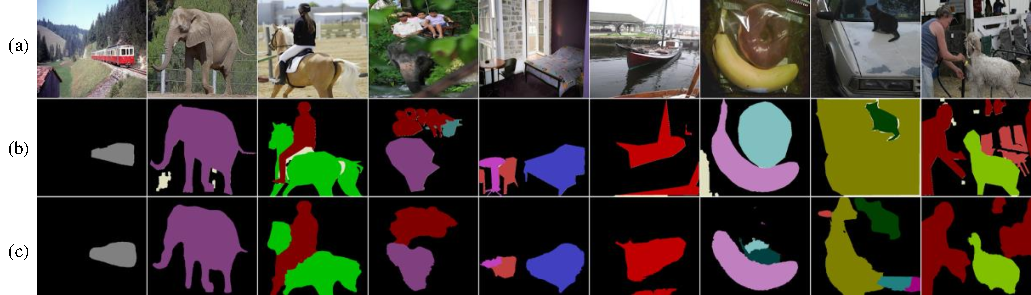
\includegraphics[width=17cm]{figures/segmentation_coco.pdf}
\caption{MS COCO 2014에서의 세분화 결과에 대한 정성적 예시입니다. (a) 입력 이미지, (b) 정답 및 (c) 우리의 EPS.}\vspace{-2mm}
\label{fig:seg_qual_coco} 
\end{figure*}


\vspace{1mm}
\noindent \textbf{세분화 맵의 정확도}. 이전 방법들~\cite{ahn2018learning, fan2020learning, wang2020self}은 의사 마스크를 생성하고 CRF 후처리 알고리즘~\cite{krahenbuhl2011efficient} 또는 친화 네트워크~\cite{ahn2018learning}로 이를 정제합니다. 한편, Table~\ref{tab:refinement}에 나타난 바와 같이, 우리가 생성한 의사 마스크는 충분히 정확하여 의사 마스크에 대한 추가 정제 없이 세분화 네트워크를 훈련합니다. 우리는 Pascal VOC 2012 데이터셋의 네 가지 세분화 네트워크에서 우리의 방법을 다른 방법들과 광범위하게 평가하고 정확하게 비교합니다.

% Please add the following required packages to your document preamble:
% \usepackage{booktabs}
\begin{table}[]
\centering
{\small
\begin{tabular}{@{}lccc@{}}
\toprule
\multicolumn{1}{c}{Method}                                                  &Seg.       &Sup.   & \multicolumn{1}{c}{val}           \\ \midrule
\multicolumn{1}{l}{SEC~\cite{kolesnikov2016seed}\textsubscript{ECCV'16}}    & V1        &I.     & \multicolumn{1}{c}{22.4}          \\
\multicolumn{1}{l}{DSRG~\cite{huang2018weakly}\textsubscript{CVPR'18}}      & V2        &I.+S.  & \multicolumn{1}{c}{26.0}          \\
\multicolumn{1}{l}{ADL~\cite{choe2020attention}\textsubscript{TPAMI'20}}    & V1        &I.+S.  & \multicolumn{1}{c}{30.8}          \\
\multicolumn{1}{l}{SGAN~\cite{yao2020saliency}\textsubscript{ACESS'20}}     & V2        &I.+S.  & \multicolumn{1}{c}{33.6}          \\ \midrule
\multicolumn{1}{l}{Our EPS}                                                 & V2        &I.+S.  & \multicolumn{1}{c}{\textbf{35.7}} \\ \bottomrule
\end{tabular}
}
\vspace{2mm}
\caption{Segmentation results (mIoU) on MS COCO 2014. All results are based on VGG16.}\vspace{-2mm}
\label{tab:seg_quantitative_coco}
\end{table}
우리의 방법은 세그멘테이션 네트워크에 관계없이 다른 방법들보다 현저히 더 나은 성능을 보입니다. Table~\ref{tab:seg_quan_voc_vgg16}은 동일한 VGG16 백본을 사용했을 때 우리의 방법이 다른 방법들보다 더 정확하다는 것을 보고합니다. 또한, VGG16에서의 우리의 결과는 더 강력한 백본(\ie Table~\ref{tab:seg_quan_voc_resnet101}의 ResNet101 기반)으로 기반한 다른 기존 방법들과 비교할 때 비슷하거나 심지어 우수합니다. 우리의 방법은 기존 방법들에 비해 명확한 개선을 보여줍니다. 마지막으로, Table~\ref{tab:seg_quan_voc_resnet101}은 우리의 방법(ResNet101 기반 DeepLab-V1과 saliency map을 사용)이 PASCAL VOC 2012 데이터셋에서 새로운 최첨단 성능(검증 세트에서 71.0, 테스트 세트에서 71.8)을 달성했음을 보여줍니다. 기존 최첨단 모델들이 달성한 이득은 약 1\%였음을 강조합니다. 반면, 우리의 방법은 이전 최고 기록보다 3\% 이상 높은 이득을 달성합니다. Figure~\ref{fig:seg_qual_voc}는 PASCAL VOC 2012에서 우리의 세그멘테이션 결과의 질적 예시를 시각화합니다. 이러한 결과는 우리의 방법이 정확한 경계를 제공하고 공존 문제를 성공적으로 해결함을 확인합니다.

Table~\ref{tab:seg_quantitative_coco}에서 우리는 COCO 2014 데이터셋에서 우리의 방법을 추가로 평가합니다. 우리는 VGG16 기반 DeepLab-V2를 세그멘테이션 네트워크로 사용하여 COCO 데이터셋에서 최첨단 WSSS 모델인 SGAN~\cite{yao2020saliency}과 비교합니다. 우리의 방법은 검증 세트에서 35.7 mIoU를 달성하며, 이는 SGAN~\cite{yao2020saliency}보다 1.9\% 높습니다. 결과적으로, 우리는 COCO 2014 데이터셋에서 새로운 최첨단 정확도를 달성합니다. 두 데이터셋에서 기존 최첨단 성능을 뛰어넘는 이러한 뛰어난 성능은 우리의 방법의 효과를 확인합니다; 지역화 맵과 saliency map을 완전히 활용하여, 목표 객체의 전체를 정확하게 포착하고 기존 모델의 단점을 보완합니다. Figure~\ref{fig:seg_qual_coco}는 COCO 2014 데이터셋에서 세그멘테이션 결과의 질적 예시를 보여줍니다. 우리의 방법은 몇 개의 객체가 가려지지 않고 나타날 때 잘 작동하지만, 많은 작은 객체를 처리하는 데는 덜 효과적입니다. 우리의 방법의 더 많은 예시와 실패 사례는 보충 자료에 제공됩니다.

\vspace{1mm}
\noindent \textbf{saliency detection 모델의 효과}. 다양한 saliency detection 모델의 효과를 조사하기 위해, 우리는 세 가지 saliency 모델을 채택합니다; PFAN~\cite{zhao2019pyramid} (우리의 기본값), OAA~\cite{jiang2019integral}와 ICD~\cite{fan2020learning}에서 사용된 DSS~\cite{hou2017deeply}, 그리고 USPS~\cite{nguyen2019deepusps} (\ie, 비지도 탐지 모델). Resnet101 기반 DeepLab-V1에서의 세그멘테이션 결과(mIoU)는 PFAN으로 71.0/71.8, DSS로 70.0/70.1, USPS로 68.8/69.9 (검증 세트와 테스트 세트)입니다. 이러한 점수는 Table~\ref{tab:seg_quan_voc_resnet101}의 다른 모든 방법보다 여전히 더 정확하다는 것을 지원합니다. 특히, 비지도 saliency 모델을 사용하는 우리의 EPS는 지도 saliency 모델을 사용하는 모든 기존 방법을 능가합니다.

\section{결론}
우리는 \emph{explicit pseudo-pixel supervision (EPS)}라는 새로운 약지도 세그멘테이션 프레임워크를 제안합니다. 지역화 맵과 saliency map 간의 상호 보완적 관계에서 영감을 받아, 우리의 EPS는 saliency map과 지역화 맵을 결합한 의사 픽셀 피드백에서 학습합니다. 우리의 공동 훈련 체계 덕분에, 우리는 양쪽의 노이즈나 누락된 정보를 성공적으로 보완합니다. 결과적으로, 우리의 EPS는 정확한 객체 경계를 포착하고 비목표 객체의 공존 픽셀을 제거하여 의사 마스크의 품질을 현저히 향상시킵니다. 광범위한 평가와 다양한 사례 연구는 우리의 EPS의 효과와 PASCAL VOC 2012 및 MS COCO 2014 데이터셋에서 WSSS에 대한 새로운 최첨단 정확도를 입증합니다.

\noindent\textbf{감사의 말씀. }
우리는 Duhyeon Bang과 Junsuk Choe에게 피드백을 주신 것에 대해 감사드립니다. 이 연구는 MSIP(과학기술정보통신부)에서 지원하는 NRF Korea의 기초과학연구프로그램(NRF-2019R1A2C2006123, 2020R1A4A1016619)과 MSIT(과학기술정보통신부)에서 지원하는 IITP(정보통신기획평가원) 지원금(2020-0-01361, 인공지능 대학원 프로그램(연세대학교)), 그리고 한국 정부에서 지원하는 한국의료기기개발기금 지원금(프로젝트 번호: 202011D06)에 의해 지원되었습니다.

{\small
\bibliographystyle{ieee_fullname}
\bibliography{egbib}
}

\end{document}
